% Backup copy of the longer XADC/UART voltage-monitor Topic 9.
% This file is intentionally not included by main.tex.

% ============================================================================
\newpage
\section{Topic 9 --- Mini oscilloscope / voltage monitor with XADC and UART}

\subsection{Background}
The AUP-ZU3 includes slow board-level analog inputs that can be read by the XADC/SYSMON path. The
on-board 10\,k$\Omega$ potentiometer and joystick are suitable signal sources for a safe lab demo. This
is a \textbf{slow voltage monitor}, not a high-speed oscilloscope: use conservative sample rates such as
100\,Hz to 1\,kHz, and expect UART bandwidth and plotting latency to dominate the experience.

\begin{notebox}
\textbf{AUP-ZU3 UART routing.} The built-in \textbf{PROG UART} COM port is connected to the Zynq
\textbf{PS} UART pins, not directly to a PL GPIO. Therefore the board-correct no-extra-hardware path is
a small PS-assisted relay: XADC/SYSMON sample in the PL, then PS UART to the PC. The RTL UART modules in
\texttt{xadc\_voltage\_monitor/src} are still useful for simulation and for boards where a PL pin is
wired to a USB-UART bridge.
\end{notebox}

The intended board data path is:
\begin{enumerate}[noitemsep]
  \item XADC/SYSMON samples the on-board analog source and produces a 12-bit ADC code
        from \texttt{0} to \texttt{4095}.
  \item A sample-rate controller chooses a slow, plot-friendly update rate such as 100\,Hz or 1\,kHz.
  \item The latest sample is exposed to the PS through a small AXI4-Lite register or FIFO.
  \item A short PS program reads the sample and prints one decimal number plus newline on PS UART1
        at 115200 baud, 8 data bits, no parity, 1 stop bit.
  \item The PC Python plotter reads the COM port and plots each incoming line as one voltage sample.
\end{enumerate}
The provided formatter and UART RTL let you simulate the serial stream format before building the full
PS-assisted board design. A direct PL-only UART can drive the PC only if a real PL pin is connected to
an external USB-UART adapter or to a board-specific UART bridge.

\begin{figure}[htbp]
  \centering
  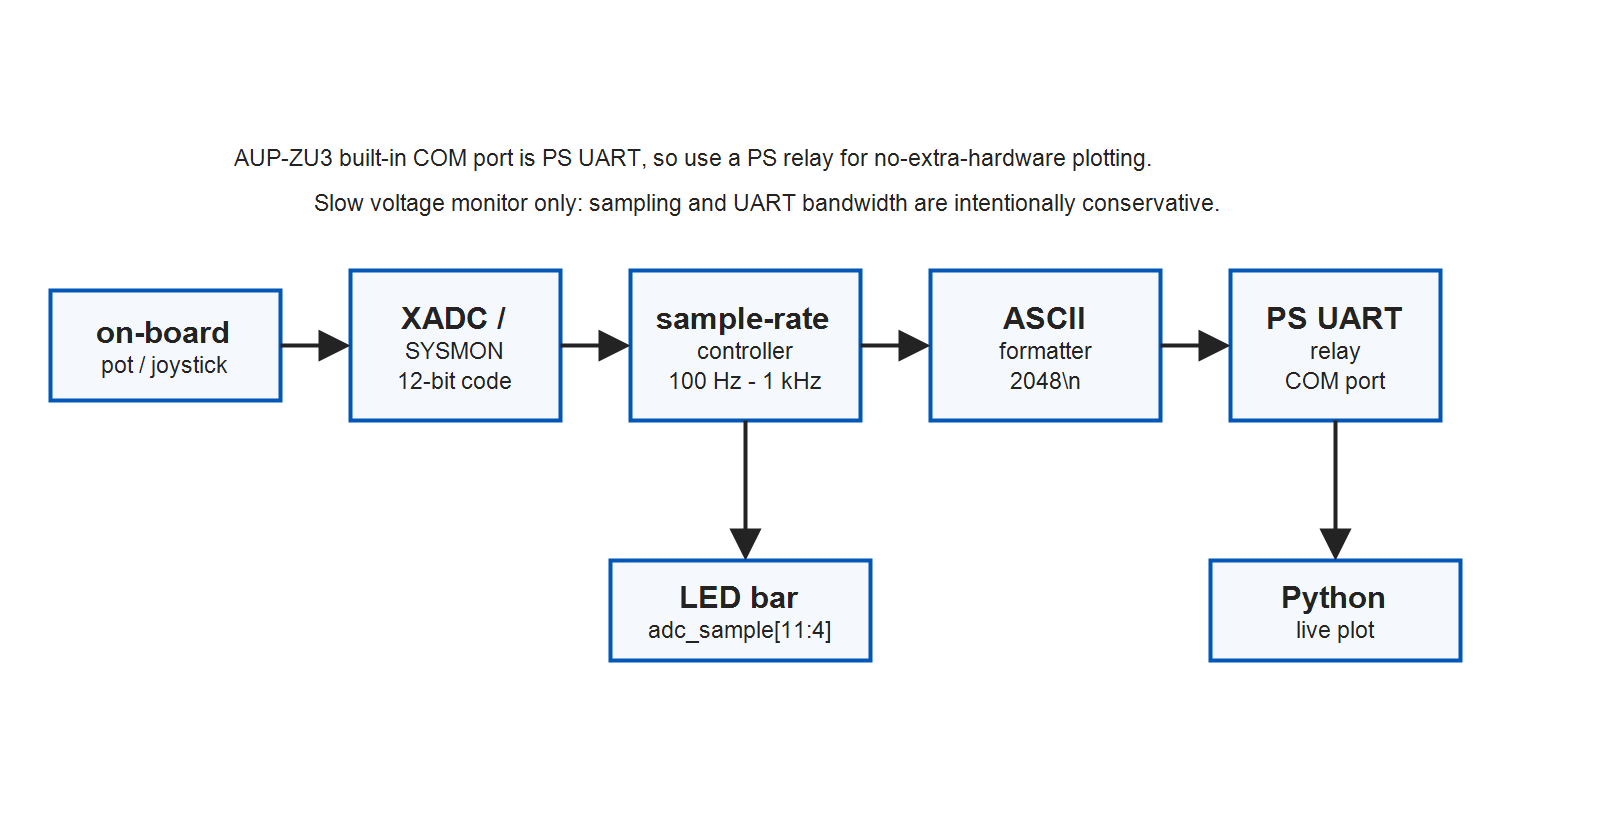
\includegraphics[width=1.0\linewidth]{Figures/screenshots/t9_01_voltage_monitor_datapath.png}
  \caption{Mini voltage-monitor data path.}
\end{figure}

\subsection{Lab 9: simulate the stream and plan the board integration}

\paragraph{Step 9.1 --- Inspect the provided RTL modules.}
Open the source files in \texttt{xadc\_voltage\_monitor/src}. The important modules are:
\begin{itemize}[noitemsep]
  \item \texttt{sample\_rate\_divider.sv}: turns the 100\,MHz PL clock into a slower sample-enable pulse.
  \item \texttt{adc\_sample\_formatter.sv}: converts a 12-bit ADC code into ASCII decimal characters
        followed by newline, for example \texttt{2048\textbackslash n}.
  \item \texttt{uart\_tx.sv}: sends one byte at a time using 115200-baud UART framing for simulation
        and optional external PL-UART bring-up.
  \item \texttt{xadc\_sysmon\_wrapper.sv}: a placeholder boundary for generated SYSMON/XADC IP. For a
        real analog board run, replace this placeholder with a Vivado-generated XADC/SYSMON instance
        connected to the on-board analog source.
  \item \texttt{top\_voltage\_monitor.sv}: a buildable PL stub that uses a ramp source so the digital
        logic can be synthesized before the real XADC and PS relay are integrated.
\end{itemize}

\paragraph{Step 9.2 --- Run the UART and formatter simulations.}
\pstag~
\begin{lstlisting}[style=ps]
vivado -mode batch -source xadc_voltage_monitor\scripts\run_voltage_monitor_simulation.tcl
\end{lstlisting}
The expected messages are \texttt{tb\_uart\_tx completed.},
\texttt{tb\_adc\_sample\_formatter completed.}, and
\texttt{INFO: Voltage-monitor module simulations complete.}

\paragraph{Step 9.3 --- Understand the AUP-ZU3 implementation choice.}
For the built-in USB-C COM port, use the PS-assisted relay described here. Generate/configure the
SYSMON/XADC block so it produces a 12-bit sample. Latch each sample at the selected sample rate, expose
the latest value to the PS through a small AXI register or FIFO, and have the PS print exactly one
decimal sample per line on PS UART1. The PC should receive lines such as:
\begin{lstlisting}[style=plain]
0
127
2048
4095
\end{lstlisting}
For a different board with a PL UART pin connected to a USB-UART bridge, the provided \texttt{uart\_tx.sv}
path can stream directly from the PL. On the AUP-ZU3 built-in PROG UART path, that direct PL-only stream
does not reach the PC because the USB-UART bridge is wired to PS MIO pins.

\paragraph{Step 9.4 --- Run the PC plotter.}
After a board design is printing one decimal ADC code per line, install the Python packages and start
the live plot:
\begin{lstlisting}[style=ps]
python -m pip install pyserial matplotlib
python xadc_voltage_monitor\python\live_plot_uart.py --port COM7 --baud 115200
\end{lstlisting}
Move the potentiometer or joystick slowly and observe the scrolling waveform.

\begin{questionbox}
\textbf{Checkpoint 9.} (1) What is the voltage resolution of a 12-bit ADC for a 1.0\,V range?
(2) Why does UART bandwidth limit the maximum sample rate? (3) Why is ASCII streaming easier to debug
but less efficient than binary streaming? (4) Why is this demo a voltage monitor rather than a true
high-speed oscilloscope?
\end{questionbox}
